\documentclass[sigconf,nonacm]{acmart}
\usepackage{xspace}
\usepackage{xcolor}
\usepackage{pgfplots}
\usepackage{subcaption}
\usepackage[capitalise,nameinlink]{cleveref}
\pgfplotsset{compat=1.16}

\usetikzlibrary{shapes.geometric}
\usetikzlibrary{arrows}
\usetikzlibrary{decorations.pathmorphing}
\usetikzlibrary{quotes}

\tikzset{every edge quotes/.style =
          { fill = white}}
          
\makeatletter
\pgfdeclareshape{document}{
\inheritsavedanchors[from=rectangle]
\inheritanchorborder[from=rectangle]
\inheritanchor[from=rectangle]{center}
\inheritanchor[from=rectangle]{north}
\inheritanchor[from=rectangle]{south}
\inheritanchor[from=rectangle]{west}
\inheritanchor[from=rectangle]{east}
\inheritanchor[from=rectangle]{north east}
\backgroundpath{
\southwest \pgf@xa=\pgf@x \pgf@ya=\pgf@y
\northeast \pgf@xb=\pgf@x \pgf@yb=\pgf@y
\pgf@xc=\pgf@xb \advance\pgf@xc by-10pt
\pgf@yc=\pgf@yb \advance\pgf@yc by-10pt
\pgfpathmoveto{\pgfpoint{\pgf@xa}{\pgf@ya}}
\pgfpathlineto{\pgfpoint{\pgf@xa}{\pgf@yb}}
\pgfpathlineto{\pgfpoint{\pgf@xc}{\pgf@yb}}
\pgfpathlineto{\pgfpoint{\pgf@xb}{\pgf@yc}}
\pgfpathlineto{\pgfpoint{\pgf@xb}{\pgf@ya}}
\pgfpathclose
\pgfpathmoveto{\pgfpoint{\pgf@xc}{\pgf@yb}}
\pgfpathlineto{\pgfpoint{\pgf@xc}{\pgf@yc}}
\pgfpathlineto{\pgfpoint{\pgf@xb}{\pgf@yc}}
\pgfpathlineto{\pgfpoint{\pgf@xc}{\pgf@yc}}
}
}
\makeatother
          
\tikzstyle{doc}=[%
draw,
thick,
align=center,
color=black,
shape=document,
minimum width=20mm,
minimum height=28.2mm,
shape=document,
inner sep=2ex,
]

\newcommand{\gearmacro}[5]{%
\foreach \i in {1,...,#1} {%
  [rotate=(\i-1)*360/#1]  (0:#2)  arc (0:#4:#2) {[rounded corners=1.5pt]
             -- (#4+#5:#3)  arc (#4+#5:360/#1-#5:#3)} --  (360/#1:#2)
}}  

\newcommand{\chaptergear}{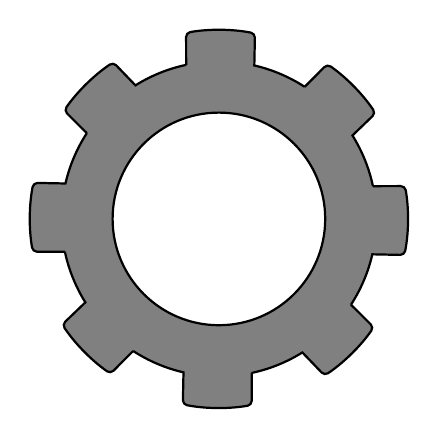
\begin{tikzpicture}
   \fill[gray] (0,0) circle (2cm);
   \draw[thick,rotate=12,fill=gray] \gearmacro{8}{2}{2.4}{20}{2};
   \draw[thick,fill=white] (0cm,0cm) circle(1.35cm);
 \end{tikzpicture}}
 
 \newsavebox\gearbox
\sbox\gearbox{\raisebox{-0.4em}{\resizebox{!}{1.5em}{\chaptergear}}}
  
\hyphenation{Web-Assembly}

\AtBeginDocument{%
  \providecommand\BibTeX{{%
    Bib\TeX}}}

\setcopyright{acmcopyright}
\copyrightyear{2024}
\acmYear{2024}
\acmDOI{XXXXXXX.XXXXXXX}

\begin{document}

\title{Wasm SpecTec: Engineering a Formal Language Standard}

\author{Joachim Breitner}
\affiliation{%
  \institution{Independent}
  \country{Germany}}
\email{mail@joachim-breitner.de}

\author{Philippa Gardner}
\affiliation{%
  \institution{Imperial College London}
  \country{United Kingdom}}
\email{p.gardner@imperial.ac.uk}

\author{Jaehyun Lee}
\affiliation{%
  \institution{KAIST}
  \country{South Korea}}
\email{99jaehyunlee@kaist.ac.kr}

\author{Sam Lindley}
\affiliation{%
  \institution{The University of Edinburgh}
  \country{United Kingdom}}
\email{Sam.Lindley@ed.ac.uk}

\author{Matija Pretnar}
\affiliation{%
  \institution{University of Ljubljana}
  \country{Slovenia}}
\email{matija.pretnar@fmf.uni-lj.si}

\author{Xiaojia Rao}
\affiliation{%
  \institution{Imperial College London}
  \country{United Kingdom}}
\email{xiaojia.rao19@imperial.ac.uk}

\author{Andreas Rossberg}
\affiliation{%
  \institution{Independent}
  \country{Germany}}
\email{rossberg@mpi-sws.org}

\author{Sukyoung Ryu}
\affiliation{%
  \institution{KAIST}
  \country{South Korea}}
\email{sryu.cs@kaist.ac.kr}

\author{Wonho Shin}
\affiliation{%
  \institution{KAIST}
  \country{South Korea}}
\email{new170527@kaist.ac.kr}

\author{Conrad Watt}
\affiliation{%
  \institution{University of Cambridge}
  \country{United Kingdom}}
\email{conrad.watt@cl.cam.ac.uk}

\author{Dongjun Youn}
\affiliation{%
  \institution{KAIST}
  \country{South Korea}}
\email{f52985@kaist.ac.kr}

%\renewcommand{\shortauthors}{TODO: we will need this}

\newcommand{\dslname}{SpecTec\xspace}
\newcommand{\todo}[1]{{\color{red}#1}}

\crefformat{section}{#2\S{}#1#3}
\crefname{figure}{Figure}{Figures}
\crefname{lstlisting}{Listing}{Listings}
\crefname{algorithm}{Algorithm}{Algorithms}
\crefname{table}{Table}{Tables}
\Crefname{line}{Line}{Lines}
\crefname{line}{line}{lines}

\begin{abstract}
WebAssembly (Wasm) is a low-level bytecode language and virtual machine, intended as a compilation target for a wide range of programming languages,  which is seeing increasing adoption across
diverse ecosystems.  As a young technology, Wasm continues to evolve --- it reached version 2.0 last year and another major update is expected soon.

For a new feature to be standardised in Wasm, four key artefacts
must be presented: a formal (mathematical) specification of the feature,  an accompanying prose pseudocode description, an implementation in the official reference
interpreter, and a suite of unit tests.
This rigorous process helps to avoid errors in the design and implementation of new Wasm features, and Wasm's distinctive formal specification in particular has facilitated machine-checked proofs of various correctness properties for the language.
 However, manually crafting all of these artefacts requires expert knowledge combined with
repetitive and tedious labor, which is a burden on the language's standardization process and authoring of the specification.

This paper presents \emph{Wasm \dslname},
a technology to express the \emph{formal} specification of Wasm through a \emph{domain-specific language}. This DSL allows all of Wasm's currently handwritten specification artefacts to be error-checked and generated automatically from a single source of truth, and is designed to be easy to write, read, compare, and review.
We believe that \emph{Wasm \dslname}'s automation and meta-level error checking will significantly ease the current burden of the language's specification authors.
We demonstrate the current capabilities of Wasm \dslname by showcasing its
proficiency in generating various artefacts, and describe our work towards replacing the manually written
official Wasm specification document with specifications generated by Wasm \dslname.
\end{abstract}

\maketitle
%!TEX root = ../main.tex

\begin{figure*}[t]
\centering
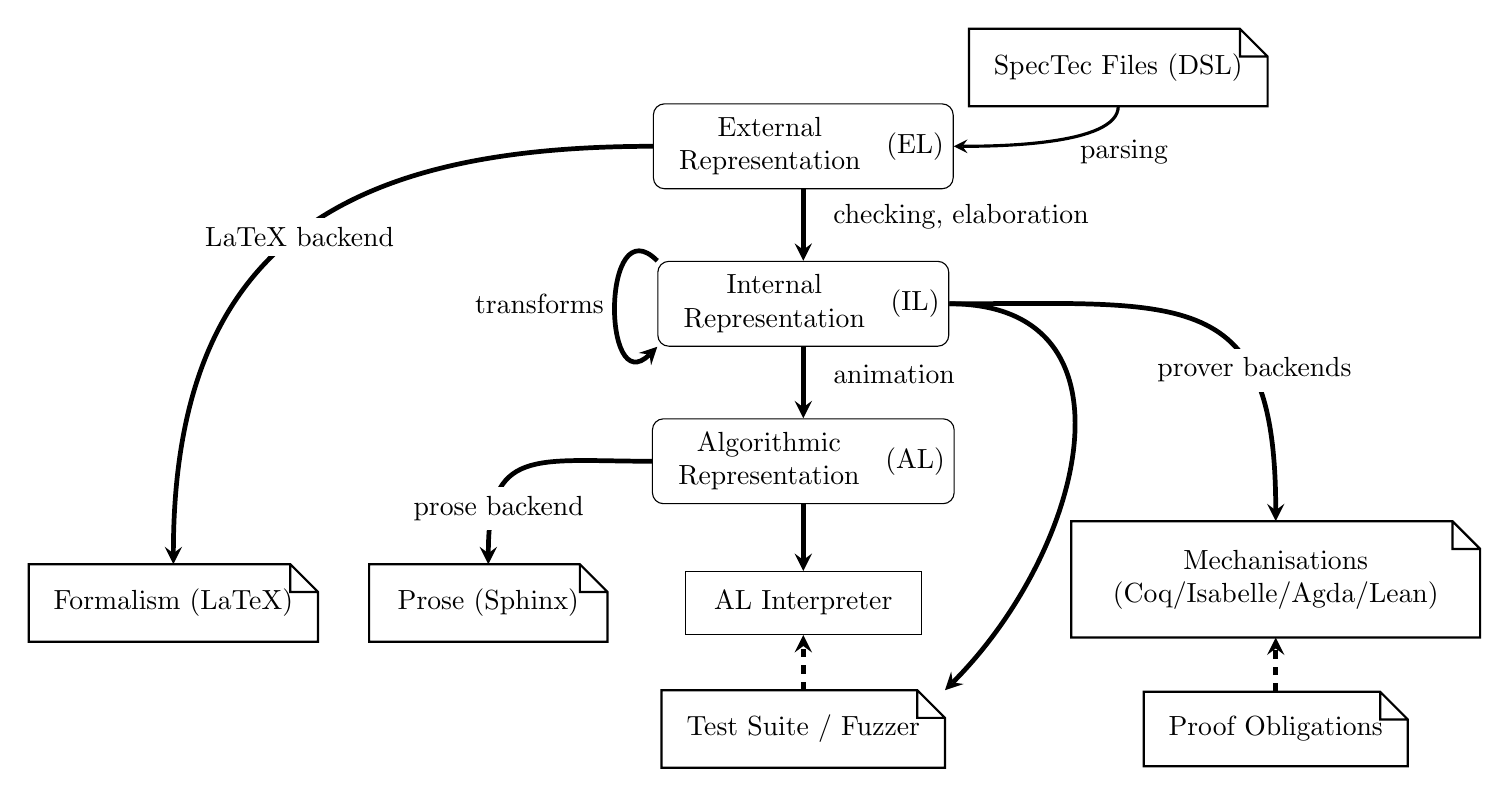
\begin{tikzpicture}

\draw (9,2) node[draw,doc, minimum height=.8cm,minimum width=3cm]
(FILES) {SpecTec Files (DSL)};

\draw (5,1) node[draw,rectangle, rounded corners, minimum height=.8cm,minimum width=3cm] (EXT) {\begin{tabular}{c}External\\Representation\end{tabular} (EL)};

\draw (5,-1) node[draw,rectangle, rounded corners, minimum height=.8cm,minimum width=3cm] (INT) {\begin{tabular}{c}Internal\\Representation\end{tabular} (IL)};

\draw (5,-3) node[draw,rectangle, rounded corners, minimum height=.8cm,minimum width=3cm] (ALG) {\begin{tabular}{c}Algorithmic\\Representation\end{tabular} (AL)};

\draw (-3,-4.8) node[draw,doc, minimum height=.8cm,minimum width=3cm] (FORM) {Formalism (LaTeX)};

\draw (1,-4.8) node[draw,doc, minimum height=.8cm,minimum width=3cm] (PROSE) {Prose (Sphinx)};

\draw (5,-4.8) node[draw,rectangle, minimum height=.8cm,minimum width=3cm] (ARINT) {AL Interpreter};

\draw (11,-4.5) node[draw,doc, minimum height=.8cm,minimum width=3cm] (MECH) {\begin{tabular}{c}Mechanisations\\(Coq/Isabelle/Agda/Lean)\end{tabular}};

\draw (5,-6.4) node[draw,doc, minimum height=.8cm,minimum width=3cm] (TEST) {Test Suite / Fuzzer};

\draw (11,-6.4) node[draw,doc, minimum height=.8cm,minimum width=3cm] (PROOF) {Proof Obligations};

\draw [line width=0.4mm, -stealth] (FILES.south) to[out=270,in=0, distance=0.5cm] node[below right, yshift=1.0ex]{\hspace{0.0em} \usebox{\gearbox} parsing} (EXT.east);
\draw [line width=0.6mm, -stealth] (EXT.south) to node[right, yshift=0.7ex]{\hspace{0.0em} \usebox{\gearbox} checking, elaboration} (INT.north);
\draw [line width=0.6mm, -stealth] (INT.south) to node[right, yshift=0.7ex]{\hspace{0.0em} \usebox{\gearbox} animation} (ALG.north);
\draw [line width=0.6mm, -stealth] (ALG.south) -- (ARINT.north);

\draw [line width=0.6mm, -stealth, dashed] (TEST.north) -- (ARINT.south);
\draw [line width=0.6mm, -stealth,dashed] (PROOF.north) -- (MECH.south);

\draw [line width=0.6mm, -stealth] (ALG.west) to[out=180,in=90, distance=1.5cm,"\usebox{\gearbox} prose backend", pos=.8] (PROSE.north);

\draw [line width=0.6mm, -stealth] (INT.east) to[out=0,in=90, distance=3cm,"\usebox{\gearbox} prover backends", pos=.7] (MECH.north);

\draw [line width=0.6mm, -stealth] (EXT.west) to[out=180,in=90, distance=4cm, "\usebox{\gearbox} LaTeX backend"] (FORM.north);

\draw [line width=0.6mm, -stealth] (INT.north west) to[out=135,in=225, distance=1cm] node[left]{\usebox{\gearbox} transforms} (INT.south west);

\draw [line width=0.6mm, -stealth] (INT.east) to[out=0,in=45, distance=2.5cm] (TEST.north east);

\end{tikzpicture}
\caption{An overview of Wasm \dslname}
\label{fig:structure}
\vspace{-0.0\baselineskip}
\end{figure*}
\section{Introduction}\label{sec:intro}
\begin{figure}[t]
  \centering
  \begin{subfigure}{\textwidth}
    \centering
    \includegraphics[width=.7\textwidth]{../img/spec-prose.png}
\vspace*{-1em}
    \subcaption{Prose notation}
\vspace*{.5em}
  \end{subfigure}
  \begin{subfigure}{\textwidth}
    \centering
    \includegraphics[width=.7\textwidth]{../img/spec-formal.png}
    \subcaption{Formal notation}
  \end{subfigure}
\caption{Semantics of \ensuremath{t.\mathit{\inblue{binop}}} in the specification}
\label{fig:spec}
\end{figure}

A programming language is defined by its syntax and semantics.
Syntax and semantics are the basis for all subsequent development and
analysis of the language, so it is important to define them clearly and rigorously. 
Many programming languages, such as Java~\cite{javaspec} and Python~\cite{pythonspec},
therefore have language specifications that define their syntax and semantics.
For languages that are prone to implementation inconsistency issues,
such as C~\cite{cstandard} and JavaScript~\cite{ecmascript},
international committees define them according to their own standardization processes.
Some languages, like Standard ML~\cite{sml}, even have formal descriptions
that define them in mathematical notation.

WebAssembly (Wasm) is a low-level bytecode language and virtual machine~\cite{wasmspec}.
It was initially designed as an efficient compilation target and execution model on Web platforms
and has been adopted across a wide range of ecosystems,
including cloud and edge computing~\cite{lucet, cloudflare}, 
mobile and embedded systems~\cite{wasm-embedded}, IoT~\cite{wasm-iot}, and
blockchains~\cite{wasm-blockchain}.
Because different browsers implement Wasm within vendor-specific architectures
using multi-tier interpretation or just-in-time compilation,
Wasm faces the risk of implementation discrepancies.
The diversity of the various ecosystems exacerbates the situation.

To mitigate these risks, Wasm has been standardized by
the W3C Wasm Community Group~\cite{wasm-w3c}.
It requires four key artifacts for a feature to be standardized:
1) a \textit{formal specification} for the feature in declarative-style rewrite rules, written in LaTeX;
2) a \textit{prose pseudocode} presenting an algorithmic-style semantics, written in reStructuredText markup;
3) an extended \textit{reference interpreter} with the implementation of the feature, written in OCaml; and
4) a \textit{unit test suite} for the feature, written in the Wasm text format.
All of these artifacts must define the same behavior of a Wasm program.
Note that the specification provides \textit{both} declarative and algorithmic styles of semantic definitions.
For example, Fig.~\ref{fig:spec} shows the execution semantics of the binary operation instruction
$t.\mathit{\inblue{binop}}$ in the official Wasm specification.
Fig.~\ref{fig:spec}(a) presents the semantics in a prose notation broken down into five steps,
while Fig.~\ref{fig:spec}(b) specifies it in a formal notation using rewrite rules.

The two styles of semantic definitions cater to the dual needs of
language ``designers'' and ``implementers.''  Declarative rewrite
rules serve the needs of designers by focusing on clarity and
correctness of language semantics. They allow theorem provers like
Coq, Isabelle, Lean, and Agda to mechanize language semantics
and prove various properties, including type safety.
Algorithmic prose pseudocode, on the other hand, helps implementers
understand language behavior. A step-by-step description of the
language semantics can be a good guide to how to implement it.

Despite the onerous standardization process, the Wasm specification has been
written and maintained \textit{manually}, which creates challenges for specification writers.
Writing the prose is extremely laborious~\cite{Andreasicfp23}, and code reviews of
feature proposals written in LaTeX and reStructuredText are not user-friendly.
Manual processes are vulnerable to human error, potentially leading
to inconsistencies or inaccuracies in the specification.
As Wasm grows with new language features such as Garbage Collected Types, Threads,
and Exception Handling that will be supported by Wasm 3.0,
manually crafting all of the artifacts is not scalable.

These challenges call for the need to automate the process or \textit{mechanize} the language semantics.
For declarative-style rewrite rules, the literature shows general-purpose language frameworks such as
Ott~\cite{ott}, PLTRedex~\cite{pltredex}, Skeleton~\cite{skeleton}, Spoofax~\cite{spoofax},
and the K framework~\cite{k}. Among them, the K framework can generate various tools,
including interpreters, model checkers, and verifiers, from a language specification written in its language K.
It has specified the core semantics of real-world programming languages
such as C~\cite{kc}, Java~\cite{kjava}, Python~\cite{kpython}, and JavaScript~\cite{kjs}.
For algorithmic-style semantics, the ESMeta framework~\cite{esmeta}
can extract a mechanized specification from
an ECMAScript/JavaScript specification~\cite{ecmascript} and automatically
generate diverse tools~\cite{jiset,jest,jstar,jsaver}.
%
%  ESMeta parses the structured English prose algorithms of ECMAScript
% Specification document, and translates them into an internal representation, $IR_{ES}$.
%   $IR_{ES}$ has its own semantics, and thus can be executed with an interpreter implementation.
%   Executing the JavaScript semantics written in $IR_{ES}$ allows an indirect execution of JavaScript programs.
%   Utilizing the executable semantics, ESMeta derives a type checker for the specification, test
% suite synthesizers, and a static analyzer of JavaScript.
%
% Now, each ECMA-262 PR will execute the ESMeta type checker, and any new or changed tests in a Test262 PR will be executed using the ESMeta interpreter.
%
ESMeta has been officially integrated into the continuous integration (CI) systems of
the ECMAScript specification~\cite{ciecma262} and the Test262 conformance test suite~\cite{citest262}
since November 2022.
Because the existing language frameworks can mechanize only one style of semantics,
they are not applicable to Wasm, which should support both declarative and algorithmic styles of semantics.

\begin{figure}[t]
\footnotesize
\begin{verbatim}
                rule Step_pure/binop-val:
                    (CONST nt c_1) (CONST nt c_2) (BINOP nt binop) ~> (CONST nt c)
                    -- if $binop(binop, nt, c_1, c_2) = c

                rule Step_pure/binop-trap:
                    (CONST nt c_1) (CONST nt c_2) (BINOP nt binop) ~> TRAP
                    -- if $binop(binop, nt, c_1, c_2) = epsilon
\end{verbatim}
\caption{The binary operator semantics in \spectec's DSL}
\label{fig:dsl}
\end{figure}

In this paper, we propose \spectec, a framework for mechanizing Wasm semantics in both styles.
\spectec presents a \emph{Domain-Specific Language (DSL)} that
defines the Wasm syntax, type system, and execution semantics in a declarative style,
which serves as a single source of truth.
Figure~\ref{fig:dsl} illustrates the semantics of $t.\mathit{\inblue{binop}}$ in the DSL,
which looks similar to the one in the official specification in Figure~\ref{fig:spec}(b).
Once the Wasm formal semantics is written in the DSL,
a number of tools can be automatically generated as backends:
1) declarative backends, including LaTeX-based formal specifications and
mechanized definitions in various theorem provers, and
2) algorithmic backends, such as prose specifications in reStructuredText and Wasm interpreters.
By conducting meta-level error checking and automatically generating the required specification artifacts,
\spectec can alleviate the burden on language designers and implementers.

\spectec's DSL is designed to provide a close and easy representation and reasoning of
the Wasm semantics in declarative backends.
It can directly produce LaTeX-based formal specifications from the definitions in the DSL,
and all definitions and variables in the DSL are ``type-checked'' to detect ill-formed ones.
It can also generate mechanized definitions for theorem provers.
This saves language designers the trouble of manually specifying
language semantics in different theorem provers every time the specification is updated.

On the contrary, algorithmic backends are not directly produced from the definitions in the DSL,
but from the definitions in the \emph{Algorithmic Language (AL)}.
The AL is designed to provide a close and easy representation and manipulation of
the Wasm semantics in the official prose specification,
so the English prose in reStructuredText markup can be generated directly from the definitions in the AL.
\spectec can also support the interpretation of Wasm programs,
following the approach of the ESMeta framework.

To bridge the gap between the two styles of semantics,
we present a mechanism for automatically deriving algorithmic ALs from declarative DSLs.
Several challenges arise in transforming declarative-style rewrite rules
into algorithmic-style prose pseudocode.
For example, a single Wasm instruction may have multiple rewrite rules,
each expressing certain premises,
but each instruction should have only one prose pseudocode. 
In addition, the equals operator `$=$' in mathematical rules
can be ambiguous, as it can mean assignment or equality checking.
We show that the transformation is an NP-hard problem
and propose a practical solution.

\spectec is available as an open-source project~\cite{spectec}
and covers everything in Wasm 2.0 except SIMD instructions.
The automatically generated Wasm semantics in the AL passes
100\% of the official test suite (except for SIMD) using an AL interpreter.
To further specify the semantics for Wasm 3.0, we only needed
to make minor adjustments in \spectec. During this process, we
reported a few errors in the Garbage Collected Types proposal and
received confirmation from the proposal champions.

This paper presents the following contributions:
\begin{itemize}
\item \textbf{\spectec is the first language semantics framework that
embraces both declarative and algorithmic styles of semantics.}
Unlike existing language frameworks that can mechanize only one style of semantics,
\spectec can support both styles of semantics.

\item \textbf{\spectec can automatically generate multiple backends from 
a single source of truth.}
It is designed to be easy to write, read, and reivew, enabling
meta-level error detection in the Wasm specification.

\item \textbf{\spectec is a forward-compatible toolchain that can
adapt to the evolving Wasm semantics.}
To evaluate \spectec's forward compatibility, we applied it to five
proposals in Wasm 3.0 and found that only minor adjustments were necessary. 
\end{itemize}

%!TEX root = main.tex

\section{Wasm \dslname}
\label{sec:structure}

An overview of Wasm \dslname is illustrated in Figure~\ref{fig:structure}.
%
The Wasm specification is primarily concerned with defining the binary format, type system, and runtime behaviour of Wasm.
%
With \dslname, an author will write these definitions in our \emph{Domain-Specific Language (DSL)}, which the Wasm \dslname toolchain accepts as input.
%
This input is parsed as the \textit{External Language (EL)} representation and processed into further representations,
namely the \textit{Internal Language (IL)} representation,
and the \textit{Algorithmic Language (AL)} representation.
Our various backends use these representations to produce the previously-described output artefacts, as well as \textit{mechanised} definitions in \textit{interactive theorem provers} suitable for machine-checked proofs about the language semantics~\cite{Watt2018MechanisingAV, Watt2021Two}.

As discussed in \cref{sec:intro}, the Wasm specification is currently written in a mixture of
reStructuredText and raw LaTeX.  Figure~\ref{fig:spec} presents the execution
semantics of the $t.\mbox{\emph{binop}}$ binary operator instruction in the Wasm specification~\cite[Section 4.4]{wasm-spec}, as rendered today.
Figure~\ref{fig:spec}(a) shows
the prose pseudocode describing the five execution steps,
and Figure~\ref{fig:spec}(b) shows the mathematics in the gray box for the corresponding
operational semantics.
%
\dslname aims to provide a significantly better developer experience without compromising on the fidelity of the rendered specification.
Moving forward, we will provide a
comprehensive breakdown of each step.

\dslname's DSL and EL are intended to closely mirror an ASCII representation of the syntactic constructs used in Wasm's formal specification.
Figure~\ref{fig:dsl} gives a DSL definition of the runtime semantics of Wasm's binary arithmetic operator,
where {\small\verb!$binop! }is a separately defined auxiliary function.
%
Crucially, all definitions and variables in the parsed EL are ``type-checked'' so that ill-formed definitions can be detected.
For example, if a specification author misses the final argument of 
{\small\verb!$binop!} as in {\small\verb!$binop(binop, nt, c_1)!},
then an arity-mismatch error will be raised.
%
From the EL, \dslname can directly produce the LaTeX-based formal specification, which is intended to replace the current specification's handwritten definitions.
Figure~\ref{fig:latex} is an excerpt from the PDF generated from the LaTeX
translated from Figure~\ref{fig:dsl}.  Compare this to the original handwritten LaTeX in Figure~\ref{fig:spec}.


To produce the other artefacts mentioned in Section~\ref{sec:intro},
the \dslname definitions are processed further.
First, the EL is elaborated into the IL, suitable for deep analysis and transformation.
Among other things, types and multiplicities of variables are inferred and annotated in the IL, mutually recursive definitions are identified, and implicit upcasts are made explicit and disambiguated.
%
As Figure~\ref{fig:structure} illustrates, the IL can undergo internal transformations to meet the needs of subsequent backends.
%
For example, in the EL expressions are modelled as
relations that can fail or can denote multiple values,  whereas various theorem prover
backends require that expressions must be purely functional, i.e.\ must denote exactly
one value given values for all free variables.
Figure~\ref{fig:lean} is an excerpt from the code generated for the Lean theorem prover~\cite{Moura2015TheLT}.
We are currently working on similarly generating code for Coq, Isabelle, and Agda.

The operational semantics of Wasm described in the IL is further transformed into the more restricted AL,
which does not allow arbitrary relational definitions and
enforces an algorithmic order of evaluation.
The problem of transforming a relational definition into an
executable, algorithmic one is known as \textit{animation}~\cite{animate}.
At its core, the process of animation involves performing a dataflow analysis on a relational definition to infer which equations of the relational definition should be interpreted as binding new variables, and ensures that these binding definitions can be ordered such that each binding definition only depends on prior animated definitions.

%!TEX root = ../main.tex

\begin{figure}[t]
  \centering
  \begin{subfigure}{\columnwidth}
    \centering
    \includegraphics[width=\columnwidth]{figs/spec-prose.png}
    \subcaption{Prose specification}
\vspace*{1em}
  \end{subfigure}

  \begin{subfigure}{\columnwidth}
    \centering
    \includegraphics[width=\columnwidth]{figs/spec-formal.png}
    \subcaption{Formal specification}
  \end{subfigure}
\caption{The binary operator semantics in the specification}
\label{fig:spec}
\end{figure}

\begin{figure}[t]
\small
\begin{verbatim}
rule Step_pure/binop-val:
  (CONST nt c_1) (CONST nt c_2) (BINOP nt binop) ~> (CONST nt c)
  -- if $binop(binop, nt, c_1, c_2) = c

rule Step_pure/binop-trap:
  (CONST nt c_1) (CONST nt c_2) (BINOP nt binop) ~> TRAP
  -- if $binop(binop, nt, c_1, c_2) = epsilon
\end{verbatim}
\caption{The binary operator semantics in \dslname's DSL}
\label{fig:dsl}
\end{figure}

\begin{figure}[t]
\small
$$
\begin{array}{@{}l@{}lcl}
{[\textsc{\scriptsize E{-}binop{-}val}]} \ \
 & (\mathit{nt}.\mathsf{const}~\mathit{c}_{1})~(\mathit{nt}.\mathsf{const}~\mathit{c}_{2})~(\mathit{nt} . \mathit{binop})
 &\hookrightarrow& (\mathit{nt}.\mathsf{const}~\mathit{c}) \\
%
& \mbox{if}~{{{\mathit{binop}}{}}_{\mathit{nt}}}{(\mathit{c}_{1},\, \mathit{c}_{2})} = \mathit{c} \\
%
{[\textsc{\scriptsize E{-}binop{-}trap}]} \ \
 & (\mathit{nt}.\mathsf{const}~\mathit{c}_{1})~(\mathit{nt}.\mathsf{const}~\mathit{c}_{2})~(\mathit{nt} . \mathit{binop})
 &\hookrightarrow& \mathsf{trap} \\
%
& \mbox{if}~{{{\mathit{binop}}{}}_{\mathit{nt}}}{(\mathit{c}_{1},\, \mathit{c}_{2})} = \epsilon
\end{array}
$$
\vspace*{-1em}
\caption{The binary operator semantics in a generated PDF}
\label{fig:latex}
\end{figure}

\begin{figure}[t]
\footnotesize
\begin{verbatim}
  | binop_val  (binop : Binop_numtype) (c : C_numtype) (c_1 : C_numtype)
               (c_2 : C_numtype) (nt : Numtype) : 
    ((«$binop» (binop, nt, c_1, c_2)) == [c]) -> 
    (Step_pure ([(Admininstr.CONST (nt, c_1)),
                 (Admininstr.CONST (nt, c_2)),
                 (Admininstr.BINOP (nt, binop))],
                [(Admininstr.CONST (nt, c))]))

  | binop_trap (binop : Binop_numtype) (c_1 : C_numtype)
               (c_2 : C_numtype) (nt : Numtype) : 
    ((«$binop» (binop, nt, c_1, c_2)) == []) -> 
    (Step_pure ([(Admininstr.CONST (nt, c_1)),
                 (Admininstr.CONST (nt, c_2)),
                 (Admininstr.BINOP (nt, binop))],
                [Admininstr.TRAP]))
\end{verbatim}
\caption{The binary operator semantics in generated Lean}
\label{fig:lean}
\end{figure}

{\sloppypar
Figure~\ref{fig:al} shows how the declarative specification of the
binary operator semantics from Figure~\ref{fig:dsl} is translated to the algorithmic version.
Note that the implicit conditions guaranteed by the Wasm validation phase
are explicitly added as assertions such as
{\small\verb!AssertI(TopValueC(NameE(nt)))!}.
Interestingly, two equality expressions are translated to different AL constructs.
Because the equality ``{\small\verb!if $binop(binop, nt, c_1, c_2) = c!}'' is a binding
that binds the result of the {\small\verb!$binop!} call to {\small\verb!c!}, it is translated as
a {\small\verb!let!} instruction:
}

\smallskip
{\small
\begin{verbatim}
    LetI(ListE([NameE(c)]),
         AppE(binop, [NameE(binop), NameE(nt),
                      NameE(c_1), NameE(c_2)]))
\end{verbatim}
}
\smallskip

\noindent
On the contrary, since ``{\small\verb!if $binop(binop, nt, c_1, c_2) = epsilon!}''
is an equality check which is inferred to bind no new variable, it is translated as a conditional expression:

\smallskip
{\small
\begin{verbatim}
    CompareC(is, AppE(binop, [NameE(binop), NameE(nt),
                              NameE(c_1), NameE(c_2)]),
             ListE([]))
\end{verbatim}
}
\smallskip

\begin{figure}[t]
\footnotesize
\begin{verbatim}
execution_of_BINOP_ainstr NameE(nt) NameE(binop):
  AssertI(TopValueC(NameE(nt)))
  PopI(ConstructE(CONST_ainstr, [NameE(nt), NameE(c_2)]))
  AssertI(TopValueC(NameE(nt)))
  PopI(ConstructE(CONST_ainstr, [NameE(nt), NameE(c_1)]))
  IfI(
    CompareC(is, LengthE(AppE(binop, [NameE(binop), NameE(nt),
                                      NameE(c_1), NameE(c_2)])), 1),
    [LetI(ListE([NameE(c)]),
          AppE(binop, [NameE(binop), NameE(nt),
                       NameE(c_1), NameE(c_2)]))
     PushI(ConstructE(CONST_ainstr, [NameE(nt), NameE(c)]))],
    [])
  IfI(
    CompareC(is, AppE(binop, [NameE(binop), NameE(nt),
                              NameE(c_1), NameE(c_2)]), ListE([])),
    [TrapI],
    [])
\end{verbatim}
\caption{The binary operator semantics in \dslname's AL}
\label{fig:al}
\end{figure}


From the AL, we directly generate a prose pseudocode specification.
Figure~\ref{fig:gen-spec} shows the prose pseudocode generated from the specification in Figure~\ref{fig:al},
which is strikingly close to the original handwritten prose description in Figure~\ref{fig:spec}.
%
We also implement an interpreter for the AL.
%
By interpreting AL that represents the Wasm semantics, we indirectly obtain an interpreter for Wasm.
%
This technique was previously used by JISET~\cite{jiset,esmeta}
to extract an executable semantics from the ECMAScript prose that represents the official
JavaScript specification~\cite{ecmascript}, and we use it here to extract an executable semantics for Wasm, from the \dslname AL.

Currently, Wasm \dslname covers all of Wasm 2.0 except for the recently-standardized SIMD vector instructions.
Within one second, our toolchain can automatically generate both prose pseudocode and operational semantics in LaTeX
with hyperlinks and cross-references in the generated PDF document, and a Lean mechanization.
We tested the extracted Wasm semantics against the official Wasm unit test suite
on an Ubuntu machine with
a 4.0GHz Intel(R) Core(TM) i7-6700k and 32GB of RAM (Samsung DDR4 2133MHz 8GB*4).
On this machine, the extracted semantics passed all 23,778 tests (SIMD excluded) in the
test suite in 21.349 seconds.

\begin{figure}[t]
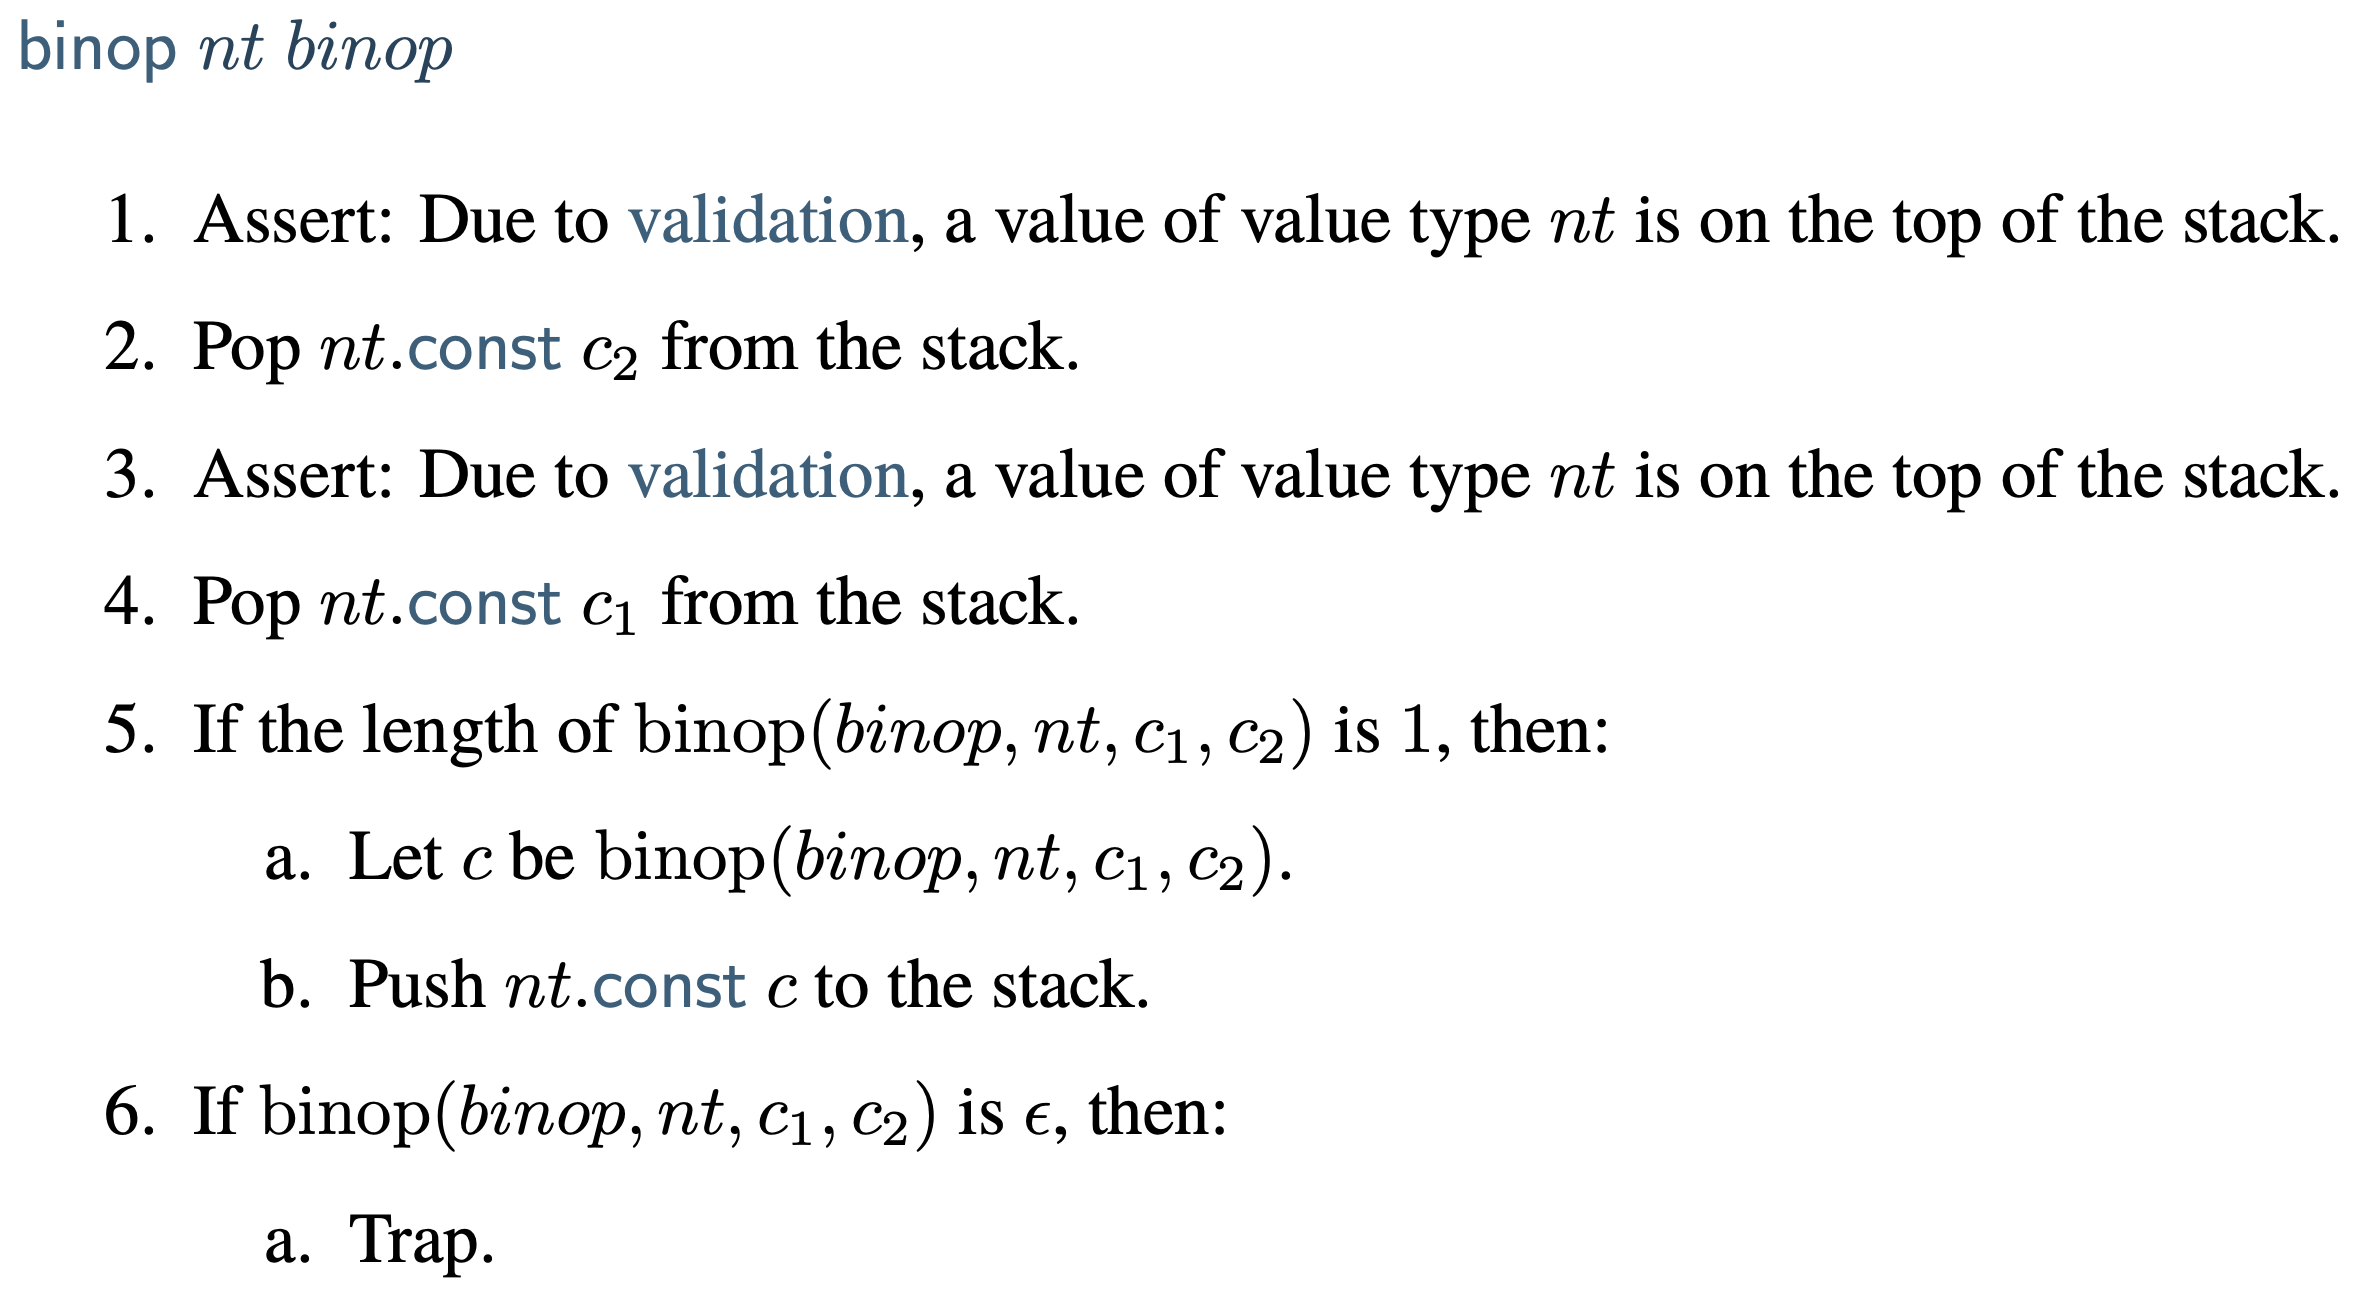
\includegraphics[width=.48\textwidth]{figs/gen-spec.png}
\caption{The binary operator semantics in generated prose}
\label{fig:gen-spec}
\end{figure}

\section{Future Plans}
\label{sec:future}

The key measure of \dslname's success is its level of adoption and ongoing support by the industrial stakeholders of the WebAssembly Community Group.
%
Our ultimate aim is for the normative definition of Wasm to be written using \dslname, and for all of the specification artefacts which are currently manually generated and maintained separately to be instead automatically generated from this \dslname definition as a single source of truth.


We now plan to gather feedback from industrial stakeholders, and evaluate how easily we can extend our definitions written in \dslname to cover additional features.
Wasm 3.0, an upcoming edition of the specification, may include Exception Handling~\cite{wasm-exc}, Garbage Collected Types~\cite{wasm-gc}, and Threads~\cite{wasm-threads}.
Because these features contain far more ambitious extensions to the Wasm virtual machine,
and are expected to lay the groundwork on which many future proposals will be built,
investigating the extent to which our \dslname definitions can be extended to cover these features would be the strongest possible validation of our approach.
%
The associated changes to the Wasm virtual machine will be wide ranging enough that we expect modifications to \dslname itself may be necessary to make it sufficiently expressive, although we are already making a best effort to anticipate the future effects of these proposals in our current design.
%
Succeeding in expressing all of these features as \dslname definitions would be a strong signal to industry stakeholders that \dslname can be seriously considered for official adoption.

%!TEX root = main.tex

\section{Conclusion}
\label{sec:conclusion}

We have presented Wasm \dslname, a technology for automatically
generating various artefacts from a single source of truth, written in the Wasm specification DSL.
We hope to replace the artefacts of the Wasm specification process
which are today onerously crafted by hand with those generated by Wasm \dslname.
This approach will facilitate the standardisation of future Wasm features
while improving the consistency and trustworthiness of Wasm's various specification artefacts. 
We also believe that \dslname will facilitate the production of trustworthy mechanizations
in diverse theorem provers, including Coq, Isabelle, Agda, and Lean.
While \dslname is still currently in development,
it is already capable of generating a formal specification and prose pseudocode covering all of Wasm 2.0 minus the SIMD instructions,
and an extracted Wasm semantics which passes all 23,778 applicable tests in the official Wasm test suite.
%
We continue to work on further backends for automatically generating unit tests and full theorem prover definitions.
%
We intend to use upcoming Wasm features such as Exception Handling,
Garbage-Collected Types, and Threads to further evaluate the utility and applicability of \dslname.
%
We acknowledge that a key challenge moving forward will be transitioning \dslname from a research tool to a robust and maintainable part of the Wasm industry standards ecosystem, and we intend to work with key Wasm industry stakeholders to achieve this goal.


\bibliographystyle{ACM-Reference-Format}
\balance
\bibliography{ref}

\end{document}
\endinput
%%
%% End of file `main.tex'.
